\documentclass{article}
\usepackage[utf8]{inputenc}
\usepackage{algorithm}
\usepackage{algorithmicx}
\usepackage[noend]{algpseudocode}
\usepackage[colorlinks=true,allcolors=blue,urlcolor={black}]{hyperref}
\usepackage[margin=1in]{geometry}
\usepackage{amsmath}
\usepackage{amssymb,amsmath,amsthm,amsfonts}
\usepackage{thmtools,bm}
\usepackage{mathtools}
\usepackage{mathrsfs}
\usepackage{tikz}
\usepackage{graphicx}
\graphicspath{{figs/}}
\usepackage{caption, subcaption}
\usepackage{booktabs}
\usepackage[numbers]{natbib}
\usepackage{smartdiagram}
\usesmartdiagramlibrary{additions} 
\usepackage{tikz}
\usetikzlibrary{arrows,quotes}
\usepackage{float}
\usepackage{parskip}
\usepackage[]{algorithm2e}

\title{CIS522 Proposal}
\author{Mingyung Kim \quad Sophie Trotto \quad Qingyun Zeng \quad Yiliang Zhang}
\date{March 2020}

\begin{document}

\maketitle

\section{Introduction}

Deep learning has infiltrated into various fields with countless applications. However, many of these tasks are expected to be operated with awareness of fairness — lawfully and without discrimination. Consider an example: an HR employee is training a deep neural network to decide whether or not an applicant should be hired. They need be cautious to make sure the decision should not be related to gender and race. As a result, the training process of the neural network involves a trade-off between fairness (non-discrimination) and quality of decision.

In general, having class balance across sensitive groups is critical in the creation of a fair algorithm. In the case of deep learning, one answer to this "trade-off" is to train a neural network while preserving group fairness is by adding a penalty term in loss function, which regularizes the fairness of the algorithms. A more extensive list of different metrics and bias mitigation algorithms has been compiled by IBM in their AI Fairness 360 toolkit \cite{aif360-oct-2018}.

Automatic facial recognition algorithms, which are used by developers including social media companies and federal law enforcement, have been shown to be biased with respect to race/ethnicity, gender, and age. A NIST study evaluated 189 software algorithms from 99 developers and found 10-100 times higher rates of false classification for (East) Asian and black faces relative to Caucasian ones. Examining only algorithms created in the U.S., the highest rate of misclassification of ethnicity was of Native Americans. Women were also less likely to be correctly identified than men, and older adults were misclassified up to 10 times more than the middle-aged  \cite{grother2019face}. Clearly, there is significant room for improvement when it comes to eliminating bias from automatic facial recognition algorithms. 

\section{Dataset}
\subsection{IMDb-Faces}
Contains 460,723 face images from 20,284 celebrities from IMDb. Attributes include gender, age, name, and year when the photo was taken \cite{Rothe-ICCVW-2015}. Notably, there is no information on race or ethnicity, which poses an issue for algorithm fairness: many face recognition models are unfair with respect to race/ethnicity because there is significant class imbalance in the dataset. More specifically, there are often many more white subjects in the dataset than subjects of other races/ethnicities — which is true of the IMDb-Faces dataset \cite{shepley2019deep}. Because we do not have label information for race or ethnicity, we cannot correct this imbalance. We are considering methods such as web scraping to find ethnicity data or using some type of proxy in order to add these labels.
\noindent The table below was constructed from a Matlab file of separate tables.
\newpage
\begin{center}
Five images from the IMDb-Faces dataset.\\
{
\includegraphics[width=0.18\textwidth]{imdb_1.jpg}}
{
\includegraphics[width=0.18\textwidth]{imdb_2.jpg}}
{
\includegraphics[width=0.18\textwidth]{imdb_3.jpg}}
{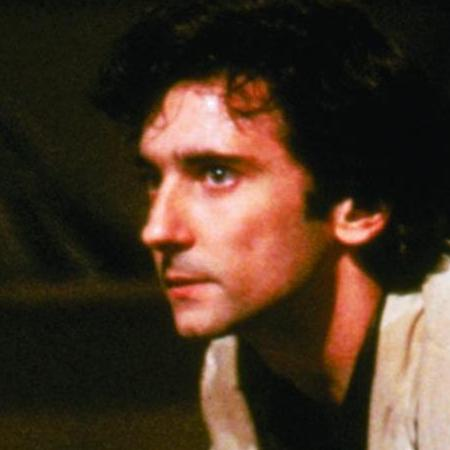
\includegraphics[width=0.18\textwidth]{imdb_4.jpg}}
{
\includegraphics[width=0.18\textwidth]{imdb_5.jpg}}
\end{center}
\begin{table}[H]
\small
\centering
\caption{Attributes of the above images (some removed for clarity).}
\begin{tabular}{llllll}
celeb\_id & name & dob & gender & photo\_taken & full\_path \\
16763 & Rowan Atkinson & 714055 & 1 & 2011 & 00/nm0000100\_rm... \\
2084 & Bill Paxton & 714186 & 1 & 2006 & 00/nm0000200\_rm... \\
10320 & Juliette Binoche & 717405 & 0 & 2005 & 00/nm0000300\_rm... \\
11878 & Linda Fiorentino & 715213 & 0 & 1985 & 00/nm0000400\_rm... \\
16119 & Richard Linklater & 716087 & 1 & 2015 & 00/nm0000500\_rm... \\
\end{tabular}
\end{table}
\noindent Interestingly, at least two of the faces (2 and 4) clearly do not match the celebrity name label. Likely, these are costars of the labelled celebrity whose faces were also tagged in their IMDB images. However, it raises the issue of inaccuracies in the dataset.
\subsection{FairFace}
Because of the lack of ethnicity data in IMDb-Faces, we also have looked at the FairFace dataset as a potential option. FairFace contains 108,501 face
images collected primarily from the YFCC-100M Flickr dataset. Attributes include age, gender, and race, and is notably balanced in distribution across the seven racial/ethnic groups represented in the dataset (White, Black, Indian, East Asian, Southeast Asian,
Middle East, and Latino)  \cite{krkkinen2019fairface}. There are no names or ids in the dataset, so it cannot be used to judge how accurately a facial recognition model can identify a person based on an image. But, because of this, FairFace does avoid the mislabelling error that IMDb-Faces has.
\begin{center} 
Five images from the FairFace training dataset.
\\
{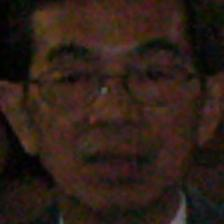
\includegraphics[width=0.18\textwidth]{fairface_1.jpg}}
{
\includegraphics[width=0.18\textwidth]{fairface_2.jpg}}
{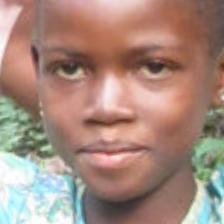
\includegraphics[width=0.18\textwidth]{fairface_3.jpg}}
{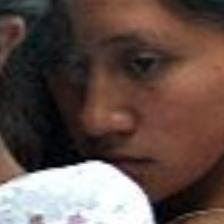
\includegraphics[width=0.18\textwidth]{fairface_4.jpg}}
{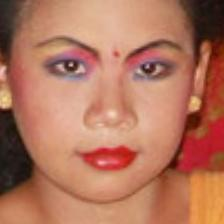
\includegraphics[width=0.18\textwidth]{fairface_5.jpg}}
\end{center}
\begin{table}[H]
\centering
\caption{Attributes of the above images.}
\begin{tabular}{lllll}
file & age & gender & race & service\_test \\
train/1.jpg & 50-59 & Male & East Asian & TRUE \\
train/2.jpg & 30-39 & Female & Indian & FALSE\\
train/3.jpg & 3-9 & Female & Black & FALSE  \\
train/4.jpg & 20-29 & Female & Indian & TRUE\\
train/5.jpg & 20-29 & Female & Indian & TRUE        
\end{tabular}
\end{table}


\section{Hypotheses}

Group fairness indicates that individuals in different groups should be treated similarly. In the setting of facial recognition, face images from different groups should be correctly classified with similar probabilities. 
\begin{itemize}
\item A normal CNN will have group unfairness.  Specifically, different groups (e.g., gender) have significantly different chance to be classified into the correct class.  Note that this hypothesis has been shown in some of the previous papers. \cite{abdurrahim2017review} \cite{michalsky2019fair} \cite{buolamwini2018gendershades}
\item With regularization on embedded feature space, our novel CNN (which we describe in the Expected Implementation/Model section) will improve group fairness. Note that this regularization may be at a cost of decreased prediction accuracy.   
\end{itemize}


\section{Inductive Biases}
As we would like to process images and identify faces, we might need translational invariance as inductive bias. In other words, we would like to build a network in a way that it would be able to recognize the class of the faces even if we translate the input images (here, face images). That is why we use CNN, which is tailored to provide translational invariance. The pooling operation (e.g., maxpooling) in CNN, which processes the nearby outputs of the convolutional layer, allows for translational invariance.   We describe our model (for now, CNN) and implementation in detail in Expected Implementation/Model section.

Another inductive bias we use is about the hidden linear layer of our novel neural network. We believe that the latent features abstract the key features of input facial images and the bias of the network is generated because of the strong associativity between some of the latent features (denote as ``biased" features) and those protected ones (e.g. gender, age and race). We then propose to eliminate these ``biased" features during predictions, which should effectively reduce the group unfairness of the network.


\section{Related Works}

\subsection{Review on The Effects of Age, Gender, and Race Demographics on Automatic Face Recognition \cite{abdurrahim2017review}}

Findings: Recognition accuracy of automatic face recognition models differs across gender, race, and age, and more strongly across interactions of these demographics. In particular, recognition accuracies of males and older people are greater than those of females and younger people.

\noindent Relevance: This paper identifies the current biases with respect to face recognition models, and what the sensitive groups of interest are.

\subsection{Deep Learning for Face Recognition: A Critical Analysis \cite{shepley2019deep}}

Findings: Contains a review of different methodologies (models, loss function, number of neural networks) for face recognition, as well as available databases. Notes, importantly, that the best models have extremely high computational cost and require large databases to provide good results.

\noindent Relevance: This paper identifies which deep learning face recognition models perform the best, which will be helpful for our group when it comes to designing our own model. It also had information on the effectiveness of the IMDB-Faces dataset, as well as the UTKFaces dataset, which overlaps significantly with FairFace.

\subsection{Fairness Criteria for Face Recognition Applications \cite{michalsky2019fair}}

Findings: Found that CNN classifier was biased against non-white individuals for gender classification despite passing standard fairness metrics. Adding confidence criteria and identifying a minimal test sample size can improve fairness.

\noindent Relevance: This paper is extremely relevant to our project, as it deals with the exact same subject: model fairness with respect to face recognition. It discusses some ways to improve fairness, which we can potentially use in our model design.

\subsection{Gender Shades: Intersectional Accuracy Disparities in Commercial Gender Classification \cite{buolamwini2018gendershades}}

Findings: While commercially-used gender-classification deep learning tools (i.e. IBM, Microsoft, and Face++) provided high classification performance on average, their error rates are significantly different across groups.  For instance, all of these tools performed worst on darker females. e  (e.g. darker males vs darker females vs lighter males vs lighter females). 


\noindent Relevance: This is one of the key papers that study group fairness in computer vision.   Our project may contribute to this research, by proposing a way to improve group fairness in facial recognition and classification.


\subsection{Fairness-aware Learning through Regularization Approach \cite{6137441}}
Findings: This paper formulates the causes of unfairness in machine learning (specifically, regression and classification) , which are categorized as 1) prejudice, 2) underestimation,  and 3) negative legacy, all of which are studied by building corresponding models on a class $Y$, a sensitive feature $X$, and a non-sensitive feature $S$. The author also proposed a method to remove unfairness caused by indirect prejudice, which was built on a regularizing method.

\noindent Relevance: This is an theory-inclined paper which build theory on how to identify causes of unfairness and the tools to identified them. We can adapt its method directly into group fairness problem into deep learning. Though it is not clear whether this might be helpful for individual fairness problem as we proposed like facial recognition. Also, the idea that how to convert definition of unfairness into statistical model and the construction of metric on quantifying the unfairness is helpful to us.

\subsection{Right for the Right Reasons: Training Differentiable Models by Constraining their Explanations\cite{ijcai2017-371}} 
Findings: In training classifier with data that are full of ambiguities, we often use regularization to narrow down choices and encourage robustness in order to get high accuracy. We usually also employ domain-specific knowledge to assist our model. But these method may not generalize well due to the confound in the data set, which might cause 'right model but wrong reasons'. The author built methods which can effectively explain and regularize differentiable model using techniques which selectively penalizing input gradient, and also with the help of expert annotation.

\noindent Relevance: This is more application-inclined than the previous paper. The mainly purpose of this paper is to get a 'right model with right reasons', which means the model we get should be consistent with knowledge in specific areas. This paper is useful for us since their technique of regularizing on specific  attributes are helpful for our research since we have similar aim. Also the dataset they use contains some vision-related ones, which also helps us to understand how the confound of the dataset can influence the model, and specifically they mentioned that their method can possibly generalize to solve problems including robustness and presence of adversarial examples.
\section{Our model}


%There are in general two types of fairness in related literature: the first one is individual fairness, which is based on the belief that similar individuals should be treated similarly. The other one is group fairness, which states members from different groups should have similar chance to achieve target outcomes. 

A widely-used definition of group fairness is statistical parity. For a decision making procedure, the statistical parity between two groups of people $a$ and $b$ is defined as:
$$
\text{SPD} = \mathcal{P}_a(\text{positive outcome}) - \mathcal{P}_b(\text{positive outcome})
$$
This quantity measures the difference of achieving positive outcomes between two different groups. there has been much literature studying how to train a neural network to guarantee group fairness. The general idea \cite{kamishima2011fairness, kamishima2012fairness} is to adds regularization term in training loss to achieve fairness:
$$
L(\theta, x, y)=\underbrace{d_{1}(y, \hat{y})}_{\text {Prediction }}+\underbrace{\lambda_{1} \mathcal{R}_f(\theta)}_{\text {Fairness }}+\underbrace{\lambda_{2} \mathcal{R}(\theta)}_{\text {Regularizer }}
$$
Where the regularization term can be set to reduce SPD of the outcomes. There are also other approaches: \cite{calmon2017optimized} uses a novel probabilistic transformation to achieve the fairness; \cite{hardt2016equality} proposes a definition of fairness and develops a post-processing step to achieve fairness. 



%To tackle this problem and make the algorithm more fair, we propose to test the performance of traditional ResNet and DenseNet on the dataset as a benchmark, then add additional fair-awared modification on the algorithms.\\


In this project, we propose $\texttt{Fair CNN}$, a new convolutional neural network structure which we anticipate to achieve group fairness. It contains a hidden linear layer which we believe to contain important latent features. To achieve group fairness, we add a penalty to those latent features that are more dependent with the protected features. We propose a novel neural network consisting of two sequential parts, the first one is a normal CNN with images as input and output a vector with predetermined length, we call these output as latent features. The second part, which is also a CNN, first do deconvolution to the input latent features, then convolve them and output the prediction result. The structure is illustrated in \hyperref[fig: 2]{figure 1}.



The intuition behind is actually inspired by autoencoders. In practice, features we use to train neural network might not be directly related to neural network. For images, each pixel is an input but it's impossible to tell which one is more related to the protected features (e.g. gender). And the first part of the network will map the input features to a lower dimensional embedded feature space. If the network has group unfairness (e.q. the SPD is too large), we anticipate that there is at least one latent feature in that layer that is strongly dependent with protected features, which we call it ``biased features".


\begin{figure}[H]
	\centering
	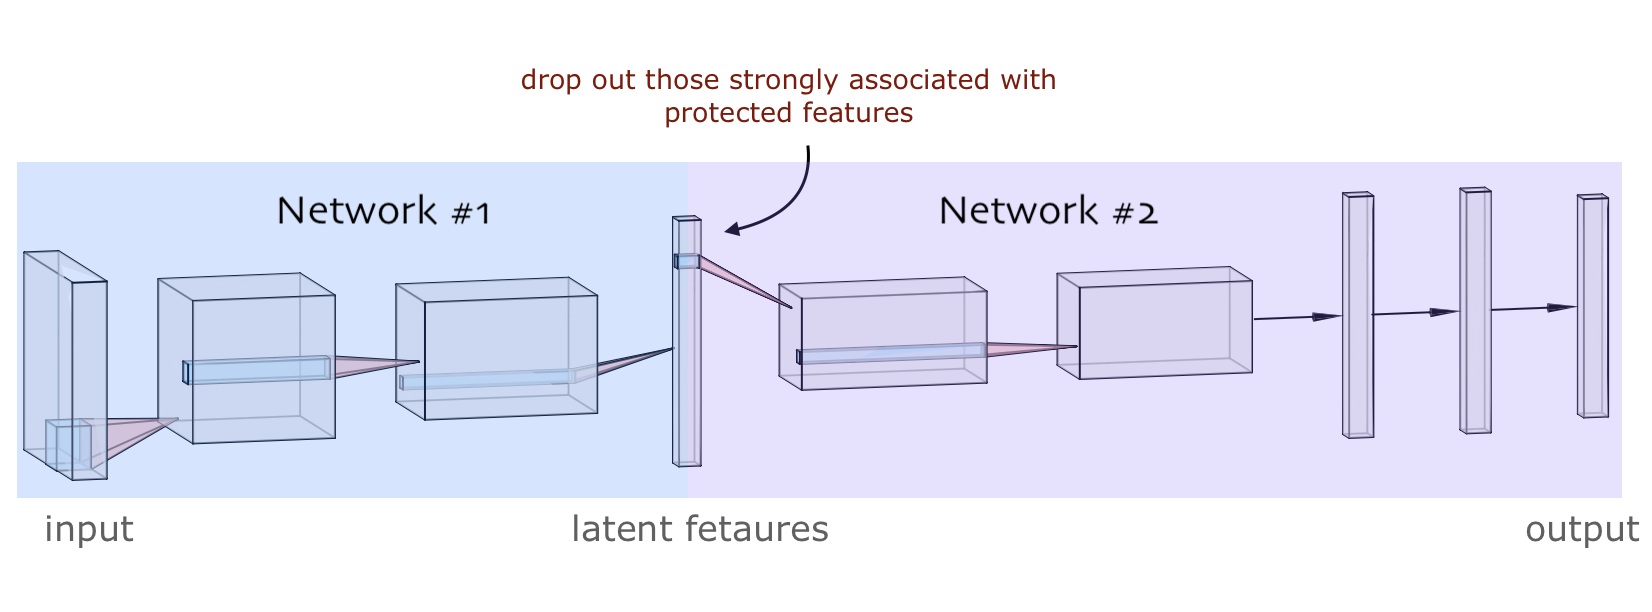
\includegraphics[width=1\textwidth]{figure/group_fair_new.png}
	%\subcaption*{3 dimensions}
	\caption{fair CNN in face recognition}
	\label{fig: 2}
\end{figure}


To remove the unfairness, we propose to eliminate those ``biased features" during model prediction step (this can be easily achieved by changing these features to the same value for every image). This way we believe that the network is only using those features irrelevant with protected ones for prediction. One potential concern is that this elimination might do harm to the prediction accuracy.




\begin{algorithm}[H]
	\KwData{facial images}
	\texttt{Network $\#$1}: output $m$ latent features using facial images
	
	\texttt{Network $\#$2}: output prediction result using $m$ latent features
	
	\KwResult{prediction of whose image}
	
	\While{training}{
		\ normally train the whole network
	}
	\ Conduct dependent test to identify ``biased'' features $\{s_1, \dots, s_k\} \subseteq \{1, \dots, m\}$ that are strongly associated with the protected features.
	
	\While{prediction}{
		\ calculate $Z = (z_1, \cdots, z_m)$, the output of \texttt{Network $\#$1} \\
		set ``biased'' features $z_{s_1}, \dots, z_{s_k}$ to be 0\\
		use \texttt{Network $\#$2} to obtain the prediction result
	}
	\caption{\texttt{Fair CNN}}
\end{algorithm}



%An alternative approach is to add penalty upon the latent features.



We can further explore this idea of removing latent biased feature on other neural network structures in computer vision field, such as ResNet and DenseNet.








\section{Timeline of Milestones}
\subsection{Milestone 1}
As a group, we will make a final selection of dataset, and do more research on available metrics — specifically, regularizing latent abstract features. Sophie will implement all of the data preprocessing, cleaning, splits, etc. so that the data is usable for the rest of the group. Mingyung will create a logistic regression baseline   for the data, Andy will create a FeedForward baseline for the data, and we will all assist Yiliang in creating a CNN baseline for the data. These baselines will represent the “unfair” models for group fairness.
\subsection{Milestone 2}
All group members will work on the novel architecture / approach discussed in our proposal to create a fair CNN Model. We will implement our novel architecture to a subset (e.g., 1000 images) of our data set, to verify that our architecture removes unfairness.
\subsection{Milestone 3}
Once we implement fair CNN model, we will calculate and compare the SPD of baselines and fair CNN and interpret the result of fair CNN. Then, we will perform hyperparameter tuning and potentially add more metrics on our novel architecture.

\newpage
\bibliographystyle{unsrt}
\bibliography{ref}

\end{document}
